\documentclass[12pt,a4paper]{report}
\usepackage{graphicx}
\usepackage{hyperref}
\usepackage{amsmath}
\usepackage{float}
\usepackage{listings}
\usepackage{color}
\usepackage{xcolor}
\usepackage{geometry}
\usepackage[many]{tcolorbox}
\usepackage{fontawesome}
\geometry{margin=1in}

% Define custom colors
\definecolor{codegray}{rgb}{0.5,0.5,0.5}
\definecolor{codepurple}{rgb}{0.58,0,0.82}
\definecolor{backcolour}{rgb}{0.95,0.95,0.92}
\definecolor{headercolor}{rgb}{0.1,0.3,0.6}
\definecolor{sectioncolor}{rgb}{0.2,0.5,0.8}

\lstdefinestyle{mystyle}{
    backgroundcolor=\color{backcolour},
    commentstyle=\color{codegray},
    keywordstyle=\color{blue},
    numberstyle=\tiny\color{codegray},
    stringstyle=\color{codepurple},
    basicstyle=\ttfamily\footnotesize,
    breakatwhitespace=false,
    breaklines=true,
    captionpos=b,
    keepspaces=true,
    numbers=left,
    numbersep=5pt,
    showspaces=false,
    showstringspaces=false,
    showtabs=false,
    tabsize=2
}

\lstset{style=mystyle}

% Define custom title style
\title{\color{headercolor}\textbf{Simple Blockchain Application: Java Project Report}}
\author{}
\date{\today}

\begin{document}

% Title page with logos and team details
\begin{titlepage}
    % Left logo (ENSA Marrakech)
    \begin{minipage}[t]{0.48\textwidth}
        \vspace{-2cm}
        \hspace{-3cm}
        
\includegraphics[width=\textwidth]{ensa_marrakech.png} % Increase the size of the logo
    \end{minipage}%
    \hfill
    % Right logo (UCA Marrakech)
    \begin{minipage}[t]{0.48\textwidth}
        \vspace{-3.5cm}
        \hspace{2.5cm}
        
\includegraphics[width=\textwidth]{uca_marrakech.png} % Increase the size of the logo
    \end{minipage}

    \vspace{1cm}

    \centering
    \Huge{\textbf{\color{headercolor} Simple Blockchain Application}}\\[1em]

    \Large{Java Project Report}\\[2em]

    % Team members' details
    \Large{Team Members:}\\
    \textbf{EL AADDAM Omar}\\
    \textbf{KHABIR Abdelhakim}\\
    \textbf{HMAMMOU Hamza}\\
    \textbf{HMIDDOUCH Abdessadek}\\
    \textbf{LOUKRISSI Meroune}\\
    \Large{Professor:}\\
    \textbf{Dr. John Professor}\\[2em]

    % University and course details
    \Large{ENSA Marrakech, Computer Science Engineering}\\[1em]
    \Large{\today}\\[2em]

    % Optional: Add a decorative line
    \rule{\textwidth}{0.4pt}\vspace{0.4cm}

    % Optional: Short description
    \large{This project involves the development of a simple blockchain application using Java, where we explore the fundamental concepts of blockchain technology and implement basic features such as mining, transaction validation, and distributed ledger management.}\\[1em]

    \vfill
    % Optional: Footer
    \large{\faUniversity\ ENSA Marrakech}
\end{titlepage}

% Set up hyperref options
\hypersetup{
    linkcolor=headercolor,
    urlcolor=sectioncolor,
    pdftitle={Blockchain Java Project Report},
}
% Enhanced Table of Contents
\renewcommand{\contentsname}{\color{headercolor}\textbf{Table of Contents}}
\tableofcontents

\chapter{Introduction to Blockchain}

Blockchain has emerged as a transformative technology, redefining how trust, transactions, and security operate in the digital age. Imagine a world where every interaction is recorded, verified, and safeguarded by a decentralized network—free from the control of a single authority. This is blockchain: a groundbreaking innovation that ensures transparency, decentralization, and security. Let us embark on a journey to explore the core principles, technologies, and applications of blockchain.

\vspace{0.5em}

\begin{tcolorbox}[colframe=black!75, colback=white, sharp corners, fonttitle=\bfseries, boxrule=0.5pt, title=\faInfoCircle\ Definition 1-1]
A \textit{Blockchain} is a system in which a record of 
transactions is maintained across several computers that are linked in a peer-to-peer network.
\end{tcolorbox}

\section{Motivation and Basic Definitions}

Let’s assume that you and your friends exchange money often, for 
example, paying for dinner or drinks. It can be inconvenient to exchange 
cash all the time. One possible solution is to keep records of all the bills that you and 
your friends have. This is called a ledger and is depicted in Figure~\ref{fig:ledger}.

\begin{figure}[h!]
    \centering
    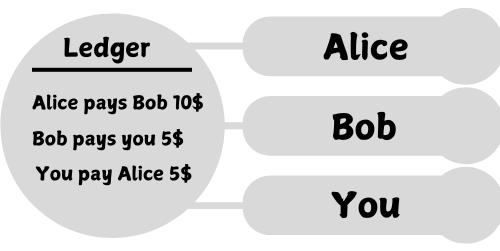
\includegraphics[width=0.8\textwidth]{ledger.png}
    \caption{A ledger and a set of connected friends (peers).}
    \label{fig:ledger}
\end{figure}

\vspace{0.5em}

\begin{tcolorbox}[colframe=black!75, colback=white, sharp corners, fonttitle=\bfseries, boxrule=0.5pt, title=\faInfoCircle\ Definition 1-2]
A \textit{ledger} is a book that contains a record of transactions.
\end{tcolorbox}

Further, at the end of every day, you all sit together and refer to the ledger to do the calculations to settle up. Let’s imagine that there is a pot 
that is the place where all of the money is kept. If you spent more than you received, you put that money in the pot; otherwise, you take that money out.

We want to design the system such that it functions similarly to a regular bank account. A holder of a wallet (bank account) should be able to only send money from their wallet to other wallets. Thus, every person in the system will have a wallet of a kind, which can also be used to determine the balance for them. Note that with the current setup using a ledger, we have to go through all the existing records to determine the balance of a specific wallet. If we want to avoid going through all the existing records, there is a way we can optimize this with unspent transaction outputs (UTXOs), as we will see later in Chapter 3.

A problem that may arise is the double-spending problem, where Bob can try to send all of his money to Alice and you at the same time, thus effectively doubling the money he sends in relation to what he owned. 

There are several ways this can be resolved, and the solution that we will provide will be a simple check of the sum of the inputs and the sum of the outputs.

A problem that might appear with this kind of system is that anyone can add a transaction. For example, Bob can add a transaction where Alice pays him a few dollars without Alice’s approval. We need to re-think our system such that each transaction will have a way to be verified/signed.

\vspace{0.5em}

\begin{tcolorbox}[colframe=black!75, colback=white, sharp corners, fonttitle=\bfseries, boxrule=0.5pt, title=\faInfoCircle\ Definition 1-3]
A \textit{digital signature} is a way to verify th
authenticity of digital messages or documents..
\end{tcolorbox}

\vspace{0.5em}

For signing and verifying transactions we will rely on digital signatures (Figure ~\ref{fig:ledd}). For now, let’s assume that anyone who adds information to the ledger also adds a signature with each record, and others have no way to modify the signature, but only to verify it. We will cover the technical details in the “Encryption” section.


\begin{figure}[H]
    \centering
    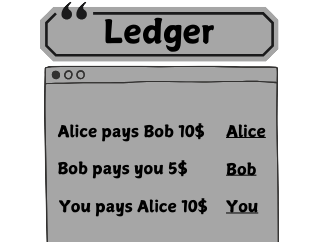
\includegraphics[width=0.8\textwidth]{ledd.png}
    \caption{Our ledger now contains signatures}
    \label{fig:ledd}
\end{figure}

\vspace{0.5em}

However, let’s assume that Bob is keeping the ledger to himself, and 
everybody agrees to this. The ledger is now stored in what is a centralized 
place. But in this case, if Bob is unavailable at the end of the day when 
everybody gathers to settle up, nobody will be able to refer to the ledger.
We need a way to decentralize the ledger, such that at any given time 
any of the people can do a transaction. For this, every person involved will 
keep a copy of the ledger to themselves, and when they meet at the end of 
the day, they will sync their ledgers.
You are connected to your friends, and so are they to you. Informally, 
this makes a peer-to-peer network.

\vspace{0.5em}

\begin{tcolorbox}[colframe=black!75, colback=white, sharp corners, fonttitle=\bfseries, boxrule=0.5pt, title=\faInfoCircle\ Definition 1-4]
A \textit{peer-to-peer} network is formed when two or more computers are connected to each other.
\end{tcolorbox}

\vspace{0.5em}

For example, when you are accessing a web page on the Internet using 
a browser, your browser is the client, and the web page you’re accessing is 
hosted by a server. This represents a centralized system since every user is 
getting the information from a single place—the server.

In contrast, in a peer-to-peer network, which represents a 
decentralized system, the distinction between a client and a server is 
blurred. Every peer is both a client and a server at the same time.

With the system (Figure ~\ref{fig:dec_ledg}), as the list of peers (people) grows, we 
might run into a problem of trust. When everybody meets at the end of 
the day to sync their ledgers, how can they believe the others that the 
transactions listed in their ledgers are true? Even if everybody trusts 
everybody else for their ledger, what if a new person wants to join this 
network? It’s natural for existing users to ask this newcomer to prove that 
they can be trusted. We need to modify our system to support this kind of 
trust. One way to achieve that is through so-called proof of work, which we 
introduce next.



\begin{figure}[H]
    \centering
    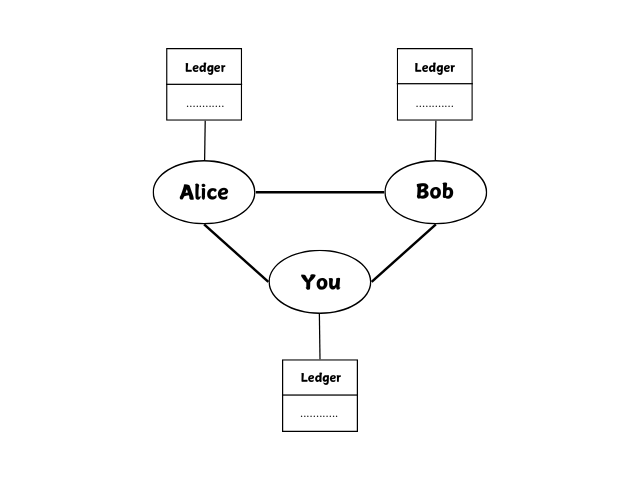
\includegraphics[width=0.8\textwidth]{dec_ledg.png}
    \caption{A decentralized ledger}
    \label{fig:dec_ledg}
\end{figure}

\vspace{0.5em}


\vspace{0.5em}

\begin{tcolorbox}[colframe=black!75, colback=white, sharp corners, fonttitle=\bfseries, boxrule=0.5pt, title=\faInfoCircle\ Definition 1-5]
A \textit{proof of work} is data that is time-consuming to calculate and easy for others to verify.
\end{tcolorbox}

\vspace{0.5em}

For each record we will also include a special number (or a hash) 
that will represent proof of work, in that it will provide proof that the 
transaction is valid. We will cover the technical details in the “Hashing” 
section.
At the end of the day, we agree that we will trust the ledger of the 
person who has put most of the work in it. If Bob has some errands to 
run, he can catch up the next day by trusting the rest of the peers in the 
network.
In addition to all this, we want the transactions to have an order, so 
every record will also contain a link to the previous record. This represents 
the actual blockchain, depicted in Figure~\ref{fig:blockchain}.

\begin{figure}[H]
    \centering
    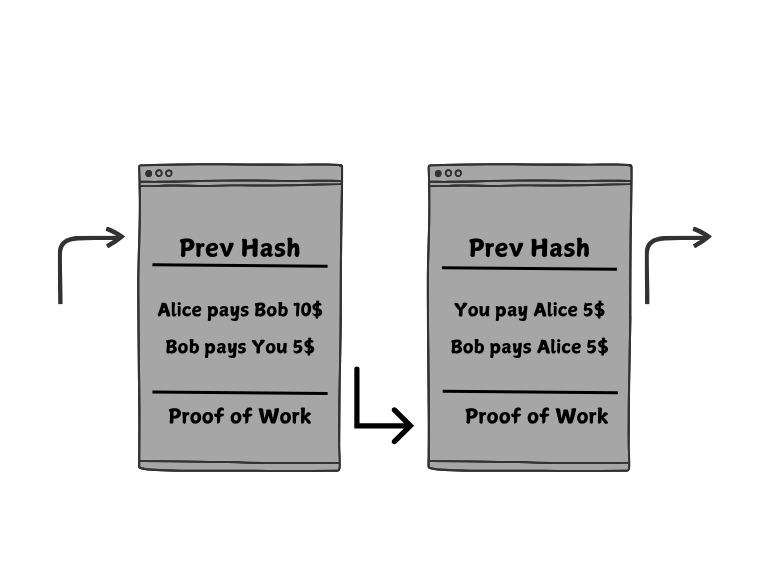
\includegraphics[width=0.8\textwidth]{blochain.png}
    \caption{A chain of blocks: blockchain}
    \label{fig:blockchain}
\end{figure}

\vspace{0.5em}

If everybody agreed to use this ledger as a source of truth, there would 
be no need to exchange physical money at all. Everybody can just use the 
ledger to put in or retrieve money from it.

To understand the technical bits of digital signatures and proof 
of work, we will be looking at encryption and hashing, respectively. 
Fortunately for us, the programming language that we will be using has 
built-in functionalities for encryption and hashing. We don’t have to dig 
too deep into how hashing and encryption and decryption work, but a 
basic understanding of them will be sufficient.

Observe how we started with a simple definition of a ledger and 
gradually built up to a complex system. We will use the same approach in 
programming.


\section{Encryption}

We will start with the following definition:

\begin{tcolorbox}[colframe=black!75, colback=white, sharp corners, fonttitle=\bfseries, boxrule=0.5pt, title=\faInfoCircle\ Definition 1-6]
\textit{Encryption} is the process of encoding information in such a way that only authorized parties can access it.
\end{tcolorbox}

\subsection{Functions}

In mathematics and computer science, a \textit{function} is a fundamental concept used to model relationships between inputs and outputs. Functions play a crucial role in encryption by transforming plaintext into ciphertext.

\begin{figure}[H]
    \centering
    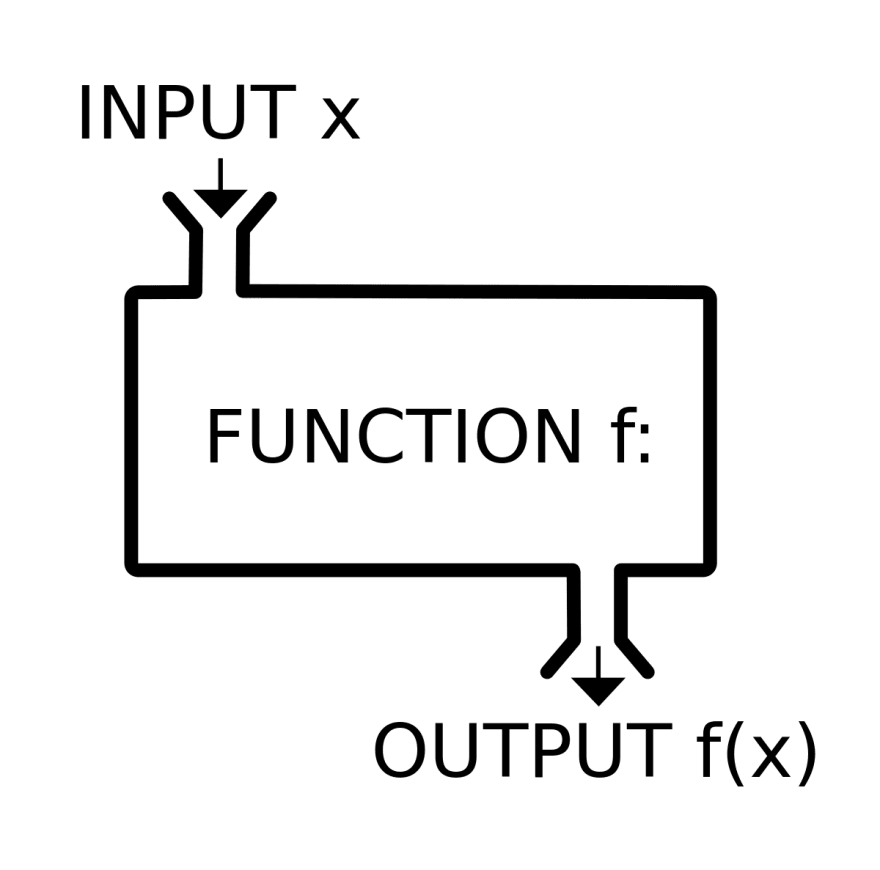
\includegraphics[width=0.5\textwidth]{function.png}
    \caption{A function}
    \label{fig:function}
\end{figure}


\begin{tcolorbox}[colframe=black!75, colback=white, sharp corners, fonttitle=\bfseries, boxrule=0.5pt, title=\faInfoCircle\ Definition 1-6]
A \textit{function} is a rule or mapping that assigns to every input exactly one output. Formally, for a function \(f(x)\), each input \(x\) from a defined domain maps to a single output \(y = f(x)\) in the codomain.
\end{tcolorbox}

To understand functions better, let’s explore some examples:

1. A function might accept a \textit{person} as input and return their \textit{name} or \textit{age} as output.

2. A mathematical function like \(f(x) = x + 1\) operates on numeric inputs:

    - If \(x = 1\), then \(f(1) = 1 + 1 = 2\).

    - If \(x = 3.14\), then \(f(3.14) = 3.14 + 1 = 4.14\).

Here’s a table illustrating this concept for \(f(x) = x + 1\):

\begin{table}[h!]
    \centering
    \begin{tabular}{|c|c|c|}
        \hline
        \textbf{Input (x)} & \textbf{Function (f(x))} & \textbf{Output (f(x))} \\ \hline
        1 & \(f(1) = 1 + 1\) & 2 \\ \hline
        2 & \(f(2) = 2 + 1\) & 3 \\ \hline
        3.14 & \(f(3.14) = 3.14 + 1\) & 4.14 \\ \hline
        10 & \(f(10) = 10 + 1\) & 11 \\ \hline
    \end{tabular}
    \caption{Example inputs and outputs for \(f(x) = x + 1\).}
    \label{table:function-example}
\end{table}


\subsection{Symmetric-Key Algorithm}

In a symmetric-key encryption system, there are two essential functions: \( E(x) \), which is the encryption function, and \( D(x) \), the decryption function. These functions must adhere to the following principles to ensure that the encryption scheme is both secure and effective:

\begin{itemize}
    \item \( E(x) \neq x \), meaning the encrypted data should be a transformed version of the original plaintext and not identical to it.
    \item \( E(x) \neq D(x) \), ensuring that the encryption and decryption processes do not produce the same result.
    \item \( D(E(x)) = x \), meaning that decrypting the encrypted message should return the original plaintext.
\end{itemize}

For instance, imagine a scenario where an encryption scheme takes the message \( E("Hello") = 4f50d1f6 \). The value "4f50d1f6" can be safely transmitted without exposing the original message. Only the intended receiver, who knows the decryption function \( D(x) \), will be able to reverse the encryption: \( D(4f50d1f6) = "Hello" \).

Another example is a shift-based encryption method, often referred to as the Caesar cipher. In this scheme, every character in the plaintext is shifted by a fixed number of positions in the alphabet. For instance, if the plaintext is "xyz", shifting each character by 3 would result in \( E("xyz") = "abc" \). To decrypt the message, the characters are shifted back by the same amount: \( D("abc") = "xyz" \).

This encryption method is a basic example of symmetric encryption, where the same function (or key) is used for both encrypting and decrypting the data. A key consideration with symmetric encryption is the secure sharing of the encryption and decryption functions between the sender and receiver, as shown in the workflow diagram in Figure~\ref{fig:symmetric-encryption}.

\begin{figure}[ht]
    \centering
    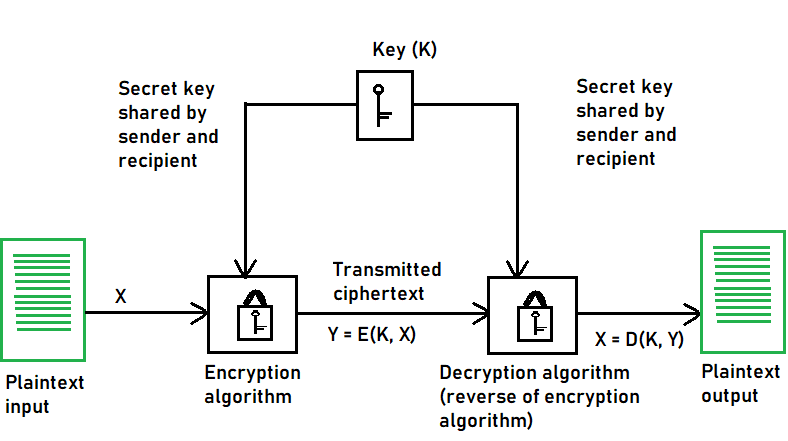
\includegraphics[width=0.75\textwidth]{symmetric-encryption.png}
    \caption{Symmetric-Key Encryption Workflow.}
    \label{fig:symmetric-encryption}
\end{figure}



\subsection{Asymmetric-Key Algorithm}

\begin{tcolorbox}[colframe=black!75, colback=white, sharp corners, fonttitle=\bfseries, boxrule=0.5pt, title=\faInfoCircle\ Definition 1-8]
An \textit{Asymmetric-Key Algorithm}, also referred to as public-key cryptography, is an encryption method that utilizes two distinct keys: a public key and a private key. The public key is used to encrypt data, while the private key is used to decrypt it, ensuring secure communication without the need for sharing the decryption key.
\end{tcolorbox}

In an asymmetric-key system, the two keys work together but are not identical. The public key can be freely distributed and used by anyone to encrypt messages intended for a specific receiver, while the private key remains confidential and is used exclusively by the receiver to decrypt the messages.

For example, let's consider an encryption scheme where Alice wants to send a secret message to Bob. Bob generates a key pair: a public key \( P_b \) and a private key \( S_b \). Bob shares his public key with Alice, but keeps his private key secure. Alice uses Bob's public key \( P_b \) to encrypt her message \( E("Hello Bob!") \), producing an encrypted ciphertext \( C \). This ciphertext can only be decrypted using Bob’s private key \( S_b \), ensuring that only Bob can read the message.

For example, let's imagine Alice wants to send a secret message to Bob. She uses Bob's public key to encrypt her message, which might look something like this:

\newline

\( E("Secure this message") = 786fbb8c4a89a3a0d7b7e7f1... \)
\newline

Now, this seemingly random string of characters is an unintelligible ciphertext to anyone who intercepts it. However, only Bob, who possesses the corresponding private key, can decrypt this message. When Bob applies his private key, the ciphertext is transformed back into the original, readable message:

\newline

\( D(786fbb8c4a89a3a0d7b7e7f1...) = "Secure this message" \)
\newline

This way, even if a malicious actor intercepts the ciphertext, they cannot read the message unless they have access to Bob's private key, which remains securely in his possession. The beauty of this process lies in how the public key ensures that anyone can send a message securely, while only the intended recipient (who holds the private key) can decrypt it and access the original content.


An example of an asymmetric encryption algorithm is RSA (Rivest-Shamir-Adleman), one of the most widely used methods. RSA relies on the mathematical difficulty of factoring large numbers. While the public key is used to encrypt data, the private key is required to decrypt it, making this method both secure and versatile for many applications, such as securing emails, online transactions, and digital signatures.
\
This asymmetric nature of encryption introduces a significant advantage over symmetric-key algorithms: the private key never needs to be shared or transmitted, reducing the risk of interception during communication. However, the system's security relies on the mathematical complexity of key generation and decryption, which requires considerable computational power.

\begin{figure}[ht]
    \centering
    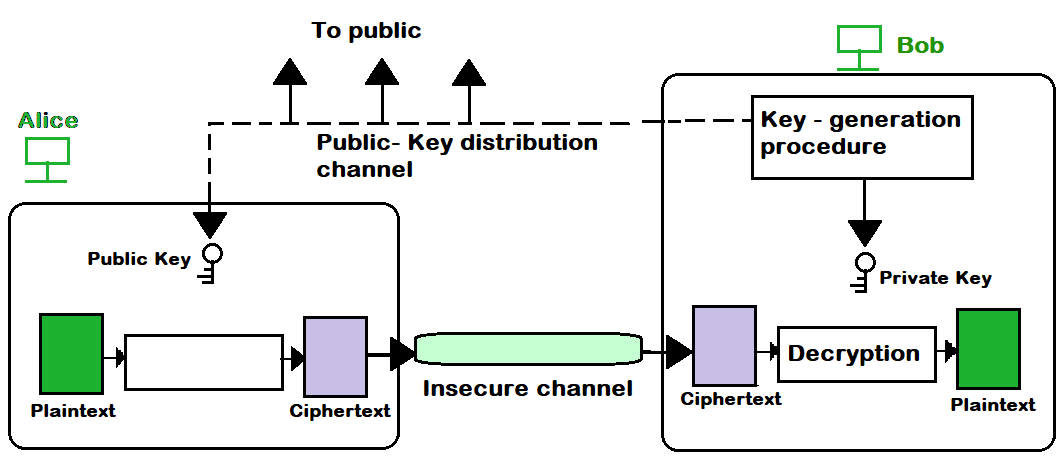
\includegraphics[width=0.75\textwidth]{asymmetric-encryption.png}
    \caption{Asymmetric-Key Encryption Workflow.}
    \label{asymmetric-encryption}
\end{figure}





\subsection{Hashing}

\begin{tcolorbox}[colframe=black!75, colback=white, sharp corners, fonttitle=\bfseries, boxrule=0.5pt, title=\faInfoCircle\ Definition 1-9: Hashing]
Hashing is a cryptographic function that transforms any input data—whether it’s a text, number, or file—into a fixed-length string, known as the hash. The crucial property of hashing is that it is \textit{one-way}: once data is hashed, it cannot be reversed back to its original form. This makes hashing ideal for securing sensitive data, verifying its integrity, and creating unique identifiers.
\end{tcolorbox}

Hashing differs significantly from encryption. While encryption can be undone using a corresponding decryption key, hashing is a one-way transformation that generates a fixed-length output, regardless of the size of the input. Because of this, it is computationally infeasible to reverse a hash and recover the original data.

For example, consider the simple hashing function that returns the length of a string:

\[
H("hello") = 5
\]
\[
H("world") = 5
\]

Notice that both "hello" and "world" yield the same hash value of 5. This is a simplified example, but it illustrates an important concept in hashing: multiple different inputs can result in the same hash, which is called a \textit{hash collision}. However, in secure cryptographic hash functions, collisions are extremely rare and hard to find.

\begin{tcolorbox}[colframe=black!75, colback=white, sharp corners, fonttitle=\bfseries, boxrule=0.5pt, title=\faInfoCircle\ Definition 1-10: Mining]
Mining refers to the process of validating transactions and adding them to the blockchain. Miners use computational resources to solve complex cryptographic problems, and in return, they are rewarded for their efforts with cryptocurrency. The process relies heavily on hashing to ensure the integrity and security of the blockchain.
\end{tcolorbox}

But why is hashing so important in systems like blockchain? Let’s dive into the fascinating world of \textit{mining} and \textit{proof of work}. Mining is essentially the computational process that powers many decentralized networks, such as Bitcoin. In this process, miners are tasked with finding a hash value that meets specific criteria, a task that requires significant computational power.

Imagine you are a miner trying to solve a cryptographic puzzle. To do this, you take a block of data and apply a cryptographic hash function to it. The goal is to find a hash that starts with a certain number of zeros (a challenge called "difficulty"). The miner who finds this hash first gets to add the block to the blockchain and is rewarded with cryptocurrency. This process is called "proof of work."


For example, if we have the block data:

\[
\text{Block Data} = \text{"Alice sends 2 BTC to Bob"}
\]

A miner will apply a hash function (e.g., SHA-256) to this data, producing a hash value. The miner then tries different variations (called "nonce") until the resulting hash meets the required difficulty level. If the hash starts with a series of zeros (e.g., 0000...), the miner has found a valid solution. The miner then broadcasts the solution to the network, and the new block is added to the blockchain.

\begin{figure}[ht]
    \centering
    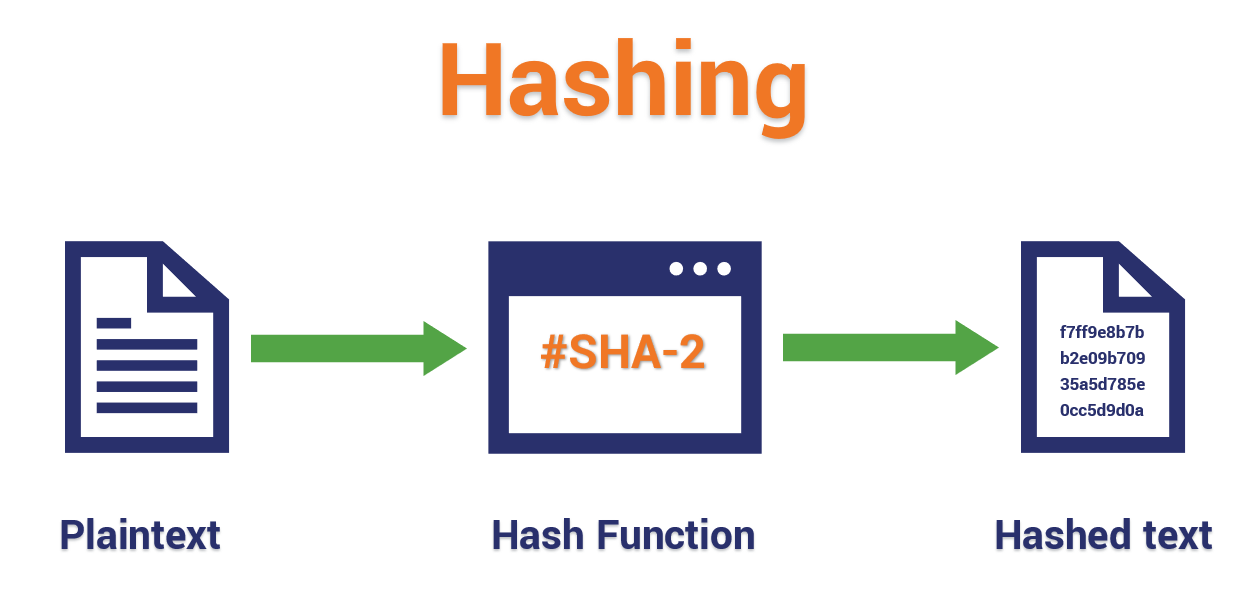
\includegraphics[width=0.75\textwidth]{hashing.png}
    \caption{SHA2 Hashing figure.}
    \label{fig:hashing}
\end{figure}

The beauty of this system lies in the fact that once a block is added to the blockchain, it is cryptographically linked to the previous block. Each block contains a hash of the previous block’s data, ensuring that any change to a block’s contents would alter its hash and invalidate the entire chain. This makes blockchain incredibly secure and resistant to tampering.

\textbf{The Power of Hashing in Blockchain:}

Hashing plays a central role in maintaining the integrity of the blockchain. It enables:

    - \textbf{Transaction Verification}: Hashing ensures that transactions in a block are valid and cannot be altered without detection.
    
    - \textbf{Proof of Work}: Mining relies on hashing to prove that a miner has expended real computational resources in solving a cryptographic puzzle.
    
    - \textbf{Linking Blocks Together}: Each block in the blockchain contains a reference to the previous block's hash, forming an unbreakable chain of verified data.
    
In summary, hashing is the backbone of many modern cryptographic systems. Whether it’s securing passwords, verifying data integrity, or powering cryptocurrency mining, hashing ensures that data remains secure, verifiable, and immutable.


\subsection{Smart Contracts}

\begin{tcolorbox}[colframe=black!75, colback=white, sharp corners, fonttitle=\bfseries, boxrule=0.5pt, title=\faInfoCircle\ Definition 1-11: Smart Contract]
A \textit{smart contract} is a self-executing contract with the terms of the agreement directly written into code. It automatically enforces and executes the terms of the contract when certain conditions are met, without the need for intermediaries or third parties. Smart contracts are primarily used in blockchain platforms to facilitate, verify, and enforce the negotiation and performance of agreements in a secure and automated manner.
\end{tcolorbox}

Smart contracts revolutionize traditional contracts by eliminating the need for manual intervention and reducing the risk of fraud or errors. Imagine a vending machine: you insert money, select your item, and the machine delivers the product. Similarly, a smart contract operates automatically once the predefined conditions are satisfied. For example, if Alice and Bob agree to exchange 10 BTC for a product, the smart contract will automatically transfer the BTC when the product is delivered, ensuring both parties fulfill their part of the agreement.

In blockchain platforms like Ethereum, smart contracts are implemented in programming languages like Solidity. They provide a decentralized, transparent way to manage transactions and business logic directly on the blockchain, making processes more efficient and secure. 

\textbf{Example:}
Consider a simple smart contract for renting a house. The contract automatically transfers the rental payment to the landlord when the tenant checks into the property. If the conditions are met (e.g., tenant's payment and check-in), the smart contract executes the transaction without any manual effort, ensuring trust and transparency.

\subsection{BetCoin}

\begin{tcolorbox}[colframe=black!75, colback=white, sharp corners, fonttitle=\bfseries, boxrule=0.5pt, title=\faInfoCircle\ BetCoin]
\textit{BetCoin} is a fictional cryptocurrency designed for online betting and gaming platforms. It leverages blockchain technology to ensure secure, transparent, and decentralized betting systems, where users can place bets and receive payouts directly through smart contracts. Unlike traditional betting systems, BetCoin eliminates intermediaries, enabling players to have complete control over their wagers and winnings.
\end{tcolorbox}

BetCoin functions as a digital asset within a decentralized betting ecosystem, allowing users to place bets in a transparent and verifiable way. Because all transactions are recorded on a blockchain, the outcome of each bet is immutable and tamper-proof, ensuring fairness. When a player wins, the corresponding amount of BetCoin is automatically transferred to their wallet through a smart contract.

For instance, in a simple betting game, Alice might wager 5 BetCoins on a coin flip. Once the flip occurs, the outcome is recorded on the blockchain, and the smart contract automatically determines whether Alice wins or loses, distributing the BetCoin based on the result.

\subsection{Example of Workflows}

In this section, we will outline a few key workflows that our system will utilize, among others.

One of the essential workflows is the \textit{mining process}. When a block is mined, a new block is created by calculating the current hash using the Hashcash algorithm. This new block contains the previous block’s hash, linking it to the existing blockchain.

When checking a wallet balance for a user (say, person A), we filter through all the blocks in the blockchain where A is either the sender or the receiver. The total balance is calculated by summing the relevant transactions. As the blockchain grows, this operation may take longer. To optimize this, we will use the \textit{Unspent Transaction Output (UTXO)} model. This model maintains a list of transactions with details on the owner and the amount of funds associated with them. Each transaction consumes entries from this list, making it more efficient to track balances.

The process of adding a block to the blockchain involves sending funds from one user (A) to another (B). To ensure that A has enough funds, we first verify the wallet balance using the workflow mentioned earlier. Once confirmed, we create a transaction (with A as the sender and B as the receiver), sign it, and then proceed to mine a block using this transaction. Finally, we update the UTXO list to reflect the rewards and the changes in the balance.


\subsection{Summary}

The aim of this chapter was to provide a broad overview of the system we will be working with. While we have laid out the foundational concepts, the next chapter will provide more explicit definitions and details for each entity.

Here’s a brief recap of what we covered in this chapter:

\begin{itemize}
    \item The key building block of our system is the \textit{block}.
    \item A block contains critical data, including transaction details.
    \item These blocks are linked together in a sequential manner to form a \textit{blockchain}, a decentralized ledger.
    \item Every participant in the system possesses a \textit{wallet} to store and manage their assets.
    \item Each transaction in the blockchain is signed by its owner, and this digital signature can be verified by anyone.
    \item The blockchain is distributed across multiple nodes, ensuring that every participant has a copy.
    \item Trust and security in the system are ensured by the \textit{proof of work} mechanism, which is integral to the mining process.
\end{itemize}





\chapter{UML Diagrams}
\section{Class Diagram}
\includegraphics[width=\textwidth]{path/to/class_diagram.png}

\section{Use Case Diagram}
\includegraphics[width=\textwidth]{path/to/use_case_diagram.png}

\section{Sequence Diagram}
\includegraphics[width=\textwidth]{path/to/sequence_diagram.png}

\chapter{Model: Blockchain Core}
\section{Block.java}
This class defines the structure of a block and includes methods for hashing and validation.
\section{Transaction.java}
Responsible for creating and verifying transactions.
\section{Wallet.java}
Handles key generation, storage, and digital signatures for transactions.
\section{Summary}
The core model ensures the blockchain's integrity and functionality.

\chapter{Database Setup}
\section{SQLite Database Browser Setup}
Steps to configure the SQLite database browser for managing blockchain data.
\section{Blockchain.db}
Schema and structure for storing the blockchain.
\section{Wallet.db}
Schema for storing wallet-related information.
\section{JDBC Driver for SQLite Setup}
Instructions to set up the JDBC driver for database connectivity.
\section{Writing Your App init() Method}
Initialization of the application with database integration.
\section{Summary}
Database setup ensures persistent and efficient data storage.

\chapter{Building the User Interface}
\section{Scene Builder Quick Setup}
Instructions to quickly set up the JavaFX Scene Builder.
\section{Creating Your Views}
\subsection{MainWindow.fxml}
Defines the main dashboard of the application.
\subsection{AddNewTransactionWindow.fxml}
Interface for adding new transactions.
\section{Creating Your View Controllers}
\subsection{MainWindowController}
Handles logic for the main dashboard.
\subsection{AddNewTransactionController}
Manages transaction creation logic.
\section{Summary}
The UI facilitates user interaction with the blockchain system.

\chapter{Network and Threads}
\section{UI Thread}
Manages the graphical interface updates.
\section{Mining Thread}
Handles block mining operations in the background.
\section{P2P Network Threads}
\subsection{PeerClient Thread}
Facilitates communication with other nodes.
\subsection{PeerServer Thread}
Listens for incoming connections.
\subsection{PeerRequestThread}
Processes peer requests in the network.
\section{Summary}
Thread management ensures smooth operation and peer-to-peer communication.

\chapter{Service Layer}
\section{WalletData}
Manages wallet-related data and operations.
\section{BlockchainData}
Handles the blockchain's state, including adding transactions and mining blocks.
\subsection{Blockchain Consensus Protocol}
Explains the consensus mechanism used in the blockchain.
\section{Summary}
The service layer integrates core functionalities with the user-facing components.

\chapter{Extras}
\section{Running the Application}
Steps to deploy and run the application successfully.
\section{Topics for Future Improvements}
\begin{itemize}
    \item Scalability enhancements.
    \item Improved consensus algorithms.
    \item Advanced security features.
\end{itemize}
\section{Conclusion}
The blockchain project demonstrates the foundational principles of distributed systems and cryptography, with room for further innovation.

\appendix

\chapter{Database Schema}
\includegraphics[width=\textwidth]{path/to/database_schema.png}

\chapter{References}
\begin{itemize}
    \item Nakamoto, S. (2008). Bitcoin: A Peer-to-Peer Electronic Cash System.
    \item Relevant textbooks and online resources.
\end{itemize}

\end{document}
